\documentclass[12pt]{article}
\usepackage[margin=1in]{geometry}
\usepackage[T1]{fontenc}
\usepackage{stix2}
\usepackage[protrusion=true,expansion=true]{microtype}
\usepackage{amsmath,amsthm}
\usepackage{graphicx}
\usepackage{booktabs}
\usepackage{threeparttable}
\usepackage[font=small,labelfont=bf,skip=4pt]{caption}
\usepackage{enumitem}
\usepackage[round,authoryear]{natbib}
\usepackage{xcolor}
\usepackage[colorlinks=true,linkcolor=black,citecolor=black,urlcolor={rgb,255:red,42;green,120;blue,214}]{hyperref}
\usepackage{xurl}
\usepackage[nameinlink,capitalise,noabbrev]{cleveref}

\setlength{\parskip}{0.2em}
\usepackage{titlesec}
\titlespacing*{\section}{0pt}{1.0em plus 0.2em}{0.45em}
\titlespacing*{\subsection}{0pt}{0.8em plus 0.2em}{0.35em}
\titlespacing*{\paragraph}{0pt}{0.45em}{0.8em}
\setlength{\textfloatsep}{12pt plus 2pt minus 2pt}
\setlength{\floatsep}{10pt plus 2pt minus 2pt}
\setlength{\parindent}{1.2em}
\setlist{itemsep=0.15em,topsep=0.3em,parsep=0pt}
\renewcommand{\arraystretch}{1.08}
\newtheorem{lemma}{Lemma}
\newcommand{\SE}{\mathrm{SE}}
\newcommand{\hb}{\hat\beta}

\title{\vspace{-1.6em}How Certain Is the Chatbot Arena Leaderboard?\\[0.2em]
\large Multiplicity, Rank Spreads and Category Specialties}
\author{Harry Hu \and Chloe Yu \and Ender Yang \and Chenxi Ge\\[0.3em]
\normalsize STAT 236 Final Project, Fall 2026}
\date{\vspace{-1.2em}}

\begin{document}
\maketitle

\begin{abstract}
\noindent Chatbot Arena ranks large language models by fitting a Bradley--Terry model to millions of pairwise human votes, and shows each model's \emph{rank spread}: the ranks consistent with per-model 95\% confidence intervals. We verify on the 2024 public battle data and on the current site that these intervals carry no multiplicity correction. In a semi-synthetic simulation that keeps Arena's real comparison graph, all 129 rank spreads hold simultaneously in 90.9\% of datasets: short of 95\%, but far better than the 0.3\% of datasets in which all score intervals hold. Every correction we study restores simultaneous coverage. Pairwise $z$-tests with Holm's step-down procedure give the narrowest valid rank intervals (11.3 ranks on average, against 13.6 for Bonferroni and 33--43 for the $\chi^2$ set of the original Arena paper), and they remain valid in stress-test worlds with exact and near ties. Category specialties are clearly present on the 2024 board: Higher Criticism, min-$P$ and $\chi^2$ all reject the null of no specialties, and Bonferroni flags 275 of 958 model--category pairs, although that count depends on how well the null's noise level is calibrated.
\end{abstract}

%====================================================================
\section{Introduction}\label{sec:intro}

Chatbot Arena (now LMArena) is the most widely cited leaderboard for large language models. A user submits a prompt, two anonymous models answer, and the user votes for the better answer. The site fits a Bradley--Terry (BT) model \citep{bradley1952rank} to these votes and ranks models by estimated strength. Since 2025 it also reports each model's \emph{rank spread}, the best and worst rank the model could hold given all models' score intervals \citep{lmarena2025ranking}. A reader who sees ``rank 2--10'' naturally takes it as a confidence statement about the rank.

The paper behind the site \citep{chiang2024arena} notes that a ranking depends on all scores at once and therefore needs simultaneous intervals; it proposes a $\chi^2$ confidence set for this. The current open-source code \citep{lmarena2025arenarank} instead computes per-model 95\% intervals $\hat r_m \pm 1.96\,\SE_m$. Plugging these into the rank-spread formula creates two errors that push in opposite directions. Without a multiplicity correction about 5\% of the intervals miss, roughly 6 of 129 models in 2024 and 20 of today's 400. But the rank spread separates two models only when their intervals do not overlap at all, which for two independent estimates with equal errors is a test at $|z| > 1.96\sqrt2 = 2.77$, the 99.4\% level. Which error wins is not known. A second question concerns Arena's category leaderboards: with about a thousand (model, category) pairs, some apparent ``specialties'' will arise by chance.

We ask: \textbf{(Q1)} how often Arena's rank spread contains the true rank, model by model and for all models at once; \textbf{(Q2)} which multiplicity-corrected procedures restore 95\% simultaneous coverage, and at what cost in width; and \textbf{(Q3)} whether category specialties exist, and which (model, category) pairs have them. True ranks are unknown on real data, so Q1 and Q2 use a semi-synthetic simulation: the BT fit on the real 2024 battles is the truth, every real matchup is kept, outcomes are redrawn, and Arena's method is rerun and checked against the true ranks. For Q3 we calibrate specialty statistics by a parametric bootstrap and compare Higher Criticism \citep{donoho2004higher} with min-$P$ and $\chi^2$ in the Rare/Weak framework.

Related work on inference for ranks includes bootstrap intervals \citep{hall2009using}, joint confidence regions for a ranking \citep{klein2020joint}, and simultaneous confidence sets built from pairwise differences with step-down testing \citep{mogstad2024inference}; our pairwise Holm procedure is the Bonferroni--Holm version of the last. We evaluate these ideas on Arena's data and comparison graph, against the procedure Arena actually uses.

%====================================================================
\section{Data and Arena's method}\label{sec:data}

\paragraph{Data.} We use the public battle dump released with \citet{chiang2024arena} \citep{lmsys2024dump} and the official leaderboard snapshot of 2024-08-12 \citep{lmarena2026dataset} as an answer key. The official filter (anonymous battles, the de-duplicated subsample, battles up to the snapshot time) leaves 1,657,517 battles among 129 models. Only 3,457 of the $\binom{129}{2} = 8{,}256$ pairs ever met, and 34.5\% of battles are ties. For the current site we use the 2026 boards in \texttt{leaderboard-dataset} and a record of what arena.ai displayed for its top 59 models on 2026-10-08.

\paragraph{Model.} Code a battle between models $i$ and $j$ as $y \in \{1, \tfrac12, 0\}$ (win, tie, loss for $i$) and write $\sigma(x) = 1/(1 + e^{-x})$. Arena's \texttt{arena-rank} package estimates strengths by the logistic loss with fractional outcomes,
\begin{equation}\label{eq:loss}
\hb = \arg\min_{\beta}\; -\sum_{\text{battles}} \bigl[\,y\,(\beta_i - \beta_j) - \log\bigl(1 + e^{\beta_i - \beta_j}\bigr)\bigr],
\end{equation}
whose target is $\mathbb E[y] = \sigma(\beta_i - \beta_j)$, and reports ratings $\hat r_m = 1000 + (400/\ln 10)\,\hb_m$. Its covariance is the sandwich estimate $\hat V = \hat H^{-1}\hat G\hat H^{-1}$ \citep{white1980heteroskedasticity}, with $\hat H$ the Hessian of \eqref{eq:loss} and $\hat G$ the covariance of the per-battle gradients. Arena's intervals are $[L_m, U_m] = \hat r_m \pm 1.96\,\SE_m$, $\SE_m = \hat V_{mm}^{1/2}$, and the rank spread is
\begin{equation}\label{eq:spread}
\text{best}_m = 1 + \#\{m' : L_{m'} > U_m\}, \qquad \text{worst}_m = 1 + \#\{m' \neq m : U_{m'} > L_m\}.
\end{equation}

\paragraph{Step 0: our Arena method is Arena's method.} Refitting the public battles with \texttt{arena-rank} reproduces the 2024 board's ratings to a median of 0.06 points. The 2024 intervals are exactly the quantiles of the 100 bootstrap fits stored in the snapshot, with a half-width of 1.90 bootstrap SDs, as expected for per-model 95\% intervals; Bonferroni or $\chi^2$ would need 3.55 or 12.42. On the current site every interval on all 4,773 published 2026 text boards is $\hat r \pm 1.9600\,\SE$, and \eqref{eq:spread} applied to the published intervals reproduces both ends of the site's rank spread for all 59 recorded models (Appendix~\ref{app:step0}). In 2024 as now, the rank spread is built from uncorrected per-model intervals.

%====================================================================
\section{Methods}\label{sec:methods}

\subsection{Semi-synthetic simulation and a reduction to orderings}\label{sec:sim}

We fit \eqref{eq:loss} once on the real battles and treat the fitted strengths $\beta^*$ as the truth, with true ranks $r_m = 1 + \#\{m' : \beta^*_{m'} > \beta^*_m\}$. Each simulated dataset keeps the same 3,457 pairs with their real battle counts and redraws the outcomes: with $p = \sigma(\beta^*_i - \beta^*_j)$ and the observed tie rate $t = 0.345$, a battle is a win, tie or loss for $i$ with probabilities $p - t/2$, $t$, $1 - p - t/2$. This keeps $\mathbb E[y] = p$, so $\beta^*$ is exactly the estimand of \eqref{eq:loss}. We refit, apply every procedure to the same fit, and repeat 1,000 times, recording per-model coverage, simultaneous coverage (all 129 intervals right), mean width, and false orderings (``$i$ above $j$'' with $\beta^*_i \le \beta^*_j$), each with a Monte Carlo standard error (Appendix~\ref{app:impl}). The following lemma, which applies to every procedure below, reduces rank intervals to declared orderings.

\begin{lemma}\label{lem:orderings}
Let a procedure declare a set $D$ of orderings ``$i$ above $j$'', and let $\text{best}_m = 1 + \#\{i : (i, m) \in D\}$ and $\text{worst}_m = M - \#\{j : (m, j) \in D\}$. For $D = \{(i, j) : L_i > U_j\}$ this is the rank spread \eqref{eq:spread}. If $D$ contains no false ordering, then $\text{best}_m \le r_m \le \text{worst}_m$ for every $m$.
\end{lemma}
\begin{proof}
If all declared orderings are true, the models declared above $m$ are among those truly above it, and those declared below $m$ are among the at most $M - r_m$ models truly below it.
\end{proof}

So any procedure whose probability of a false ordering is at most 5\% has simultaneous rank coverage of at least 95\%. A false ordering needs two models with nearly equal strengths: a score interval that misses does no harm unless it crosses a close neighbour's.

\subsection{Corrected procedures (Q2)}\label{sec:procs}

\Cref{tab:procs} lists when each procedure declares $i$ above $j$. Bonferroni and the $\chi^2$ set keep Arena's overlap rule and widen the intervals. The $\chi^2$ set of \citet{chiang2024arena}, $\{\beta : (\hb - \beta)^\top\hat V^{-}(\hb - \beta) \le \chi^2_{M-1,\,0.95}\}$, projects onto each coordinate as $\hb_m \pm 12.47\,\SE_m$; read through pairwise contrasts \citep{scheffe1953method} it declares $i$ above $j$ when $\beta_i > \beta_j$ on the whole set. The pairwise procedures test each pair directly with
\[
z_{ij} = \frac{\hat r_i - \hat r_j}{\SE(\hat r_i - \hat r_j)}, \qquad \SE(\hat r_i - \hat r_j)^2 = \hat V_{ii} + \hat V_{jj} - 2\hat V_{ij}.
\]
In these units the overlap rule demands $|z_{ij}| > 1.96\,\rho_{ij}$ with $\rho_{ij} = (\SE_i + \SE_j)/\SE(\hat r_i - \hat r_j)$. On the real fit $\rho_{ij}$ ranges from 1.09 to 1.73 (median 1.37); it exceeds $\sqrt2$ when estimates are positively correlated, as for models that play each other often or face the same opponents. Pairwise Bonferroni uses $z_{1-\alpha/(2K)} = 4.52$ for all $K = 8{,}256$ pairs. Holm \citep{holm1979simple} compares the $k$-th largest $|z|$ with $z_{1-\alpha/(2(K-k+1))}$, stops at the first failure, and declares each rejected pair in the direction of $z_{ij}$. One-sided Holm applies Holm's procedure to the $2K$ hypotheses $H_{ij}: \beta_i \le \beta_j$, whose rejection is exactly the ordering ``$i$ above $j$''; its $k$-th bar is $z_{1-\alpha/(2K-k+1)}$, which never falls below $z_{1-\alpha/(K+1)} = 4.38$.

\begin{table}[t]
\centering\small
\caption{When each procedure declares model $i$ above model $j$ (gap $= \hat r_i - \hat r_j$; $M = 129$, $K = 8{,}256$, $\alpha = 0.05$). ``Proven'': the probability of any false ordering is at most $\alpha$ under any dependence, up to the normal approximation.}\label{tab:procs}
\begin{tabular}{@{}lll@{}}
\toprule
Procedure & Rule & False orderings controlled \\
\midrule
Arena (uncorrected) & gap $> 1.96\,(\SE_i + \SE_j)$ & none \\
Bonferroni intervals & gap $> 3.55\,(\SE_i + \SE_j)$ & proven \\
$\chi^2$ projection & gap $> 12.47\,(\SE_i + \SE_j)$ & proven \\
$\chi^2$ Scheff\'e & $z_{ij} > 12.47$ & proven \\
Pairwise Bonferroni & $z_{ij} > 4.52$ & proven \\
Holm (two-sided) & $z_{ij} >$ step-down bar, 4.52 falling toward 1.96 & exact ties only \\
Holm (one-sided) & $z_{ij} >$ step-down bar, 4.52 falling to $\ge$ 4.38 & proven \\
\bottomrule
\end{tabular}
\end{table}

\paragraph{Guarantees.} By \cref{lem:orderings} the quantity to control is the probability of a false ordering. Bonferroni-type rules bound it by the union bound. Holm's theorem bounds the chance of rejecting any \emph{true} hypothesis, which for the one-sided version are exactly the false orderings. For the textbook two-sided Holm, exactly tied pairs are true nulls and are covered, but a close, untied pair is a false null whose possible error is a wrong \emph{direction}. Directional control after a two-sided Holm is proven for independent statistics under conditions normal ones meet \citep{shaffer1980control}; our $z_{ij}$ are never independent, since pairs share models, and for dependent statistics the question is open \citep{finner1999stepwise, guo2016directional}. We test it empirically below. A proof buys little here: each pair always keeps one true one-sided hypothesis, so declaring orderings never reduces the number of ways to be wrong. Finally, all three pairwise procedures declare exactly the pairs with $|z|$ above a cutoff; because $\SE(\hat r_i - \hat r_k) \le \SE(\hat r_i - \hat r_j) + \SE(\hat r_j - \hat r_k)$, declaring $i > j$ and $j > k$ implies $z_{ik} \ge \min(z_{ij}, z_{jk})$, so their orderings are always transitive.

\paragraph{Benchmark and stress tests.} As an oracle benchmark we recompute rank spreads from $\hb \pm z\,\SE$ for $z \in [1.8, 4]$ and find the smallest $z$ reaching 95\% simultaneous coverage; it needs the true ranks, so it is not a procedure. To probe the guarantees where they bind, we rerun the simulation on the same graph with changed strengths: all strengths scaled by 0.5, 0.25, 0.1 or 0; models sorted into 20 or 10 tiers of exactly equal strength (354 or 768 tied pairs); and 20 tiers in which each model keeps 5\%, 10\% or 20\% of its distance from the tier mean (median within-tier gap 0.1--0.4 standard errors). In the last three worlds every error is a wrong direction, the unproven case.

\subsection{Category specialties (Q3)}\label{sec:q3methods}

We define eight categories from the dump's prompt tags (coding, math, instruction following, hard prompts, Chinese, Russian, multi-turn, long query); each reproduces the official 2024 board of the same name (Appendix~\ref{app:q3}). We test the $N = 958$ (model, category) pairs with at least 200 category battles. For model $m$ in category $c$, with $y_b$ its score in battle $b$ and $p_b = \sigma(\hb_m - \hb_{o(b)})$ the win probability implied by the \emph{overall} fit,
\[
z_{mc} = \textstyle\sum_b (y_b - p_b) \big/ \sqrt{\sum_b (y_b - p_b)^2}
\]
over $m$'s battles in $c$. Because the overall fit uses these battles too, $z_{mc}$ is shrunk toward zero and the $z_{mc}$ are correlated. We therefore calibrate by a parametric bootstrap under the null of no specialties (redraw all outcomes from the overall fit and refit, 500 times); the raw null SDs range from 0.70 to 1.05. Each $z_{mc}$ is standardized against its null mean and SD to $z^*_{mc}$, with two-sided $p$-values from $N(0,1)$.

To ask whether \emph{any} specialty exists we use Higher Criticism, $\mathrm{HC} = \max_{k \le N/2} \sqrt N\,(k/N - p_{(k)})/\sqrt{p_{(k)}(1 - p_{(k)})}$, its variant HC$^+$ restricted to $p_{(k)} > 1/N$, min-$P$ ($\max|z^*|$) and $\chi^2 = \sum z^{*2}$, each with a $p$-value from the null draws. To ask \emph{which}, we use Bonferroni (family-wise 5\%) and Benjamini--Hochberg \citep{benjamini1995controlling} (FDR 10\%). For power we plant $s = N^{1-\vartheta}$ specialties of strength $\mu = \sqrt{2r\log N}$ in $z$ units \citep{donoho2015higher}, $\vartheta \in \{0.2, \dots, 0.7\}$, $r \in \{0.1, \dots, 1.5\}$, 200 replicates per cell, with critical values from fresh null draws.

%====================================================================
\section{Results}\label{sec:results}

\subsection{Q1: the rank spread is nearly right, by cancellation}\label{sec:q1}

\begin{figure}[t]
\centering
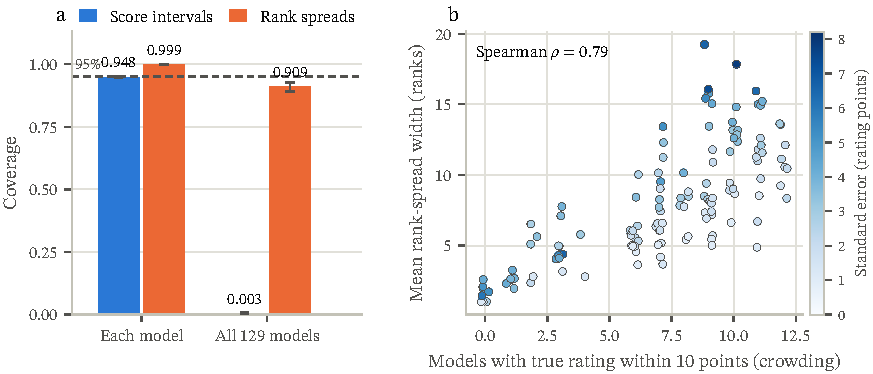
\includegraphics[width=\textwidth]{figures/fig1_q1.pdf}
\caption{Q1, 1,000 simulated datasets. (a) Coverage of Arena's score intervals and rank spreads, for each model and for all 129 at once, with 95\% Monte Carlo intervals. (b) Mean rank-spread width of each model against the number of models with true rating within 10 points, colored by standard error.}\label{fig:q1}
\end{figure}

Each score interval covers its true score 94.8\% of the time, but on average 6.65 of the 129 miss, and all 129 cover in only 3 of 1,000 datasets (\cref{fig:q1}a). The rank spreads are far more robust: each contains its true rank 99.9\% of the time, and all 129 do so in $90.9\% \pm 0.9\%$ of datasets. Only 103 of the 129,000 simulated rank spreads missed. The shortfall from 95\% is 4.5 Monte Carlo SEs: real, but small.

The two errors nearly cancel. A missed score interval rarely changes a rank (\cref{lem:orderings}), and the overlap rule's conservatism absorbs most of the remaining misses. The result is too conservative for a single model and slightly anti-conservative for the whole table. Nothing in the method targets either level, so the 91\% should move with the number of models, their spacing and the amount of data. The simulated spreads match the real ones in width (8.0 against 7.9 ranks).

The main driver of rank instability is crowding (\cref{fig:q1}b): the number of models within 10 rating points has Spearman correlation 0.79 with the spread width, against 0.27 for the standard error and 0.23 for the true rank, and in a joint regression strength is not significant ($t = 1.1$). Spreads are widest for true ranks 61--100 (12.1 ranks), where models are densest (Appendix~\ref{app:q1}).

\subsection{Q2: pairwise tests with Holm give the narrowest valid rank intervals}\label{sec:q2}

\begin{figure}[t]
\centering
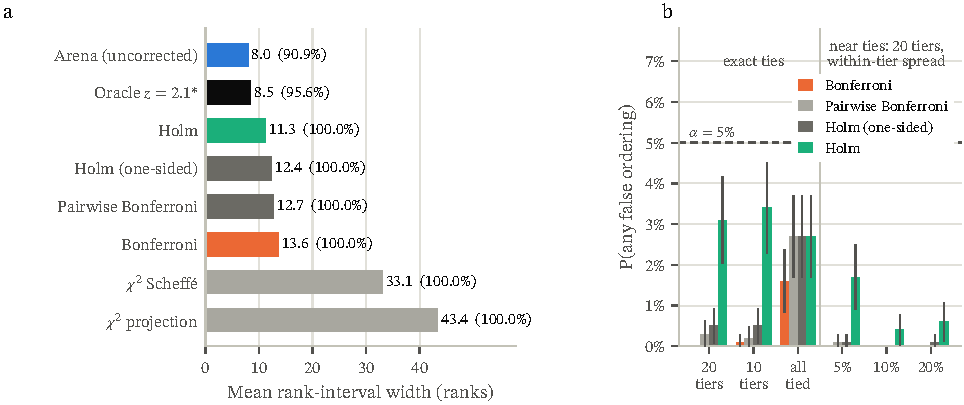
\includegraphics[width=\textwidth]{figures/fig2_q2.pdf}
\caption{Q2. (a) Mean rank-interval width on the 1,000 datasets of Q1; in parentheses, the share of datasets in which all 129 intervals contain the true ranks. *The oracle chooses $z$ using the true ranks. (b) Probability of any false ordering in the stress-test worlds (1,000 datasets each), with 95\% Monte Carlo intervals; the dashed line is the 5\% target.}\label{fig:q2}
\end{figure}

Every correction reaches 100\% simultaneous coverage without a single false ordering, but the costs differ fourfold (\cref{fig:q2}a). The $\chi^2$ set is by far the most expensive (33.1 ranks read through contrasts, 43.4 projected): it protects every linear combination of the 129 scores, and its multiplier $\sqrt{\chi^2_{128,0.95}} = 12.47$ grows like $\sqrt M$, whereas a ranking only needs the signs of $K$ differences, for which $\sqrt{2\log K}$ suffices. Bonferroni intervals need 13.6 ranks. Pairwise Holm needs 11.3, 18\% less, and detects 92.0\% of the true orderings against Bonferroni's 90.1\%.

The gain has two sources. Testing each gap directly saves 0.9 ranks (13.6 to 12.7): the overlap rule inflates a gap's uncertainty by $\rho_{ij} \approx 1.37$, which costs more than the move from $M$ to $K$ tests (3.55 to 4.52) adds. Holm's step-down saves 1.5 more: about 7,600 pairs are rejected, many with $|z| > 20$, so the bar for the rest falls from 4.52 to 3.96. The one-sided Holm, whose control is proven, reaches only 12.4 because its bar stops at 4.38. All corrections still overshoot: the oracle reaches 95.6\% at $z = 2.1$ with 8.5 ranks.

\paragraph{Stress tests.} A false ordering needs a pair whose true gap $\delta$ (in SEs) is near zero, since its probability is about $\Phi(-\delta - \text{bar})$; the 2024 strengths have few such pairs, while family-wise bounds are built for many exact ties. \Cref{fig:q2}b shows the worlds where the bounds bind. With 20 or 10 exactly tied tiers, Holm's bar falls to 3.96--4.01 and it declares a false ordering in 3.1\% and 3.4\% of datasets, against at most 0.5\% for procedures with a fixed or slowly falling bar. This matches the bar: a tied pair clears 3.96 with probability $7.6 \times 10^{-5}$, and $354 \times 7.6 \times 10^{-5} = 2.7\%$. With all models tied the three pairwise procedures coincide at 2.7\%, below 5\% because the 8,256 statistics are positively correlated. In the near-tie worlds, the unproven case, Holm's error rate falls to 1.7\%, 0.4\% and 0.6\% as the spread grows, and its coverage stays at or above 99.4\%. Exact ties, which Holm's theorem covers, are the hardest case. Arena's uncorrected spreads collapse once ties exist: all hold in 24\%, 7\% and 0.2\% of datasets with 20 tiers, 10 tiers and all models tied (Appendix~\ref{app:q2}).

\begin{figure}[t]
\centering
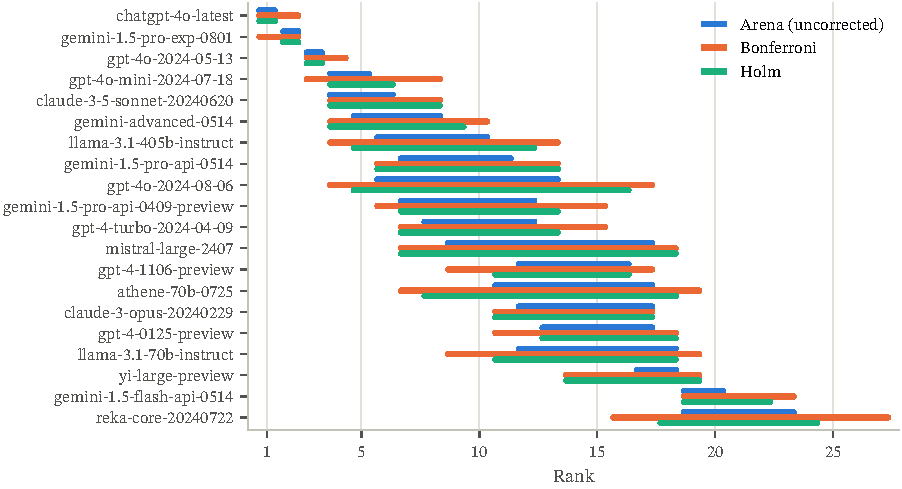
\includegraphics[width=0.84\textwidth]{figures/fig3_q2_real.pdf}
\caption{Rank intervals of the 20 highest-rated models on the 2024 board (our refit of the public battles).}\label{fig:real}
\end{figure}

\paragraph{The real 2024 board.} Holm keeps each of the top three models at a single rank, as Arena does, whereas Bonferroni ties the top two (\cref{fig:real}). The mean width over all 129 models is 7.9 for Arena, 11.4 for Holm and 13.8 for Bonferroni. Of the 7,808 orderings Arena declares, Holm does not support 223, with $|z|$ between 2.5 and 3.96: significant one at a time but not among 8,256 comparisons. They involve 117 models, mostly in the crowded lower half of the table. Conversely, Holm separates no pair that Arena shows as tied, whether a tie means overlapping score intervals (448 pairs) or overlapping rank spreads, the site's rule (830 pairs): Arena's implicit bar $1.96\,\rho_{ij}$ lies between 2.1 and 3.4, always below 3.96. A max-$|z|$ test using the exact correlations of the 8,256 statistics would need a bar of 4.30 instead of 4.52, and its step-down version \citep{romano2005exact} separates only 18 more pairs than Holm, so Holm captures most of what a family-wise procedure can gain here.

\subsection{Q3: category specialties are real, but their number is uncertain}\label{sec:q3}

\begin{figure}[t]
\centering
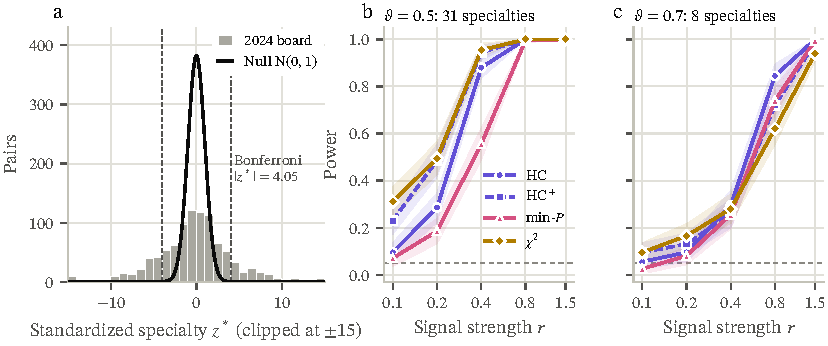
\includegraphics[width=\textwidth]{figures/fig4_q3.pdf}
\caption{Q3. (a) Standardized specialty statistics $z^*$ of the 958 tested pairs on the 2024 board against the null $N(0,1)$; dashed lines mark the Bonferroni bar. (b, c) Power of the global tests for many ($\vartheta = 0.3$) and few ($\vartheta = 0.7$) planted specialties, 200 replicates per point; dotted line: 5\%.}\label{fig:q3}
\end{figure}

\begin{table}[t]
\centering\small
\caption{Q3 on the 2024 board: $N = 958$ tested pairs; null distribution from 500 parametric-bootstrap draws (smallest attainable $p = 1/501$).}\label{tab:q3}
\begin{tabular}{@{}lrrr@{\hspace{2em}}lr@{}}
\toprule
Global test & Observed & Null 95\% point & $p$ & Identification & Pairs flagged \\
\midrule
HC$^+$ & 330 & 3.1 & $< 0.002$ & Bonferroni (FWER 5\%) & 275 \\
$\chi^2$ & 21{,}210 & 1{,}028 & $< 0.002$ & BH (FDR 10\%) & 525 \\
min-$P$ ($\max|z^*|$) & 40.3 & 4.05 & $< 0.002$ & naive $p < 0.05$ & 521 \\
HC & $1.2 \times 10^{62}$ & 4.4 & $< 0.002$ & \quad expected by chance & 48 \\
\bottomrule
\end{tabular}
\end{table}

The 2024 category effects are far from the null (\cref{fig:q3}a, \cref{tab:q3}). Every global test rejects at the smallest attainable $p$-value, and Bonferroni flags 275 pairs, in every category (17--40\% of its pairs) and for 94 of the 129 models, with median size 25 rating points. The largest are language effects: \texttt{llama-3-70b-instruct} is 73 points weaker in Chinese than overall ($z^* = -40$), and all nine Qwen models are 50--84 points stronger, eight significantly. Plain HC is about $10^{62}$ because the smallest $p$-value underflows to zero and is dropped, leaving the second smallest ($2.8 \times 10^{-127}$) to dominate; HC$^+$ is the usable version.

Whether specialties exist is settled; how many is not. The null redraws battles independently, ignoring correlated votes (same user or session, time clusters) and BT misfit. On the real board the $z^*$ have a robust SD of 3.3 rather than 1. If the true noise were 1.5, 2 or 3 times the null's, Bonferroni would flag 149, 76 or 26 pairs instead of 275.

The power simulation (\cref{fig:q3}b,c) reproduces the ordering of the Rare/Weak theory, on a narrow range. With many specialties ($\vartheta = 0.3$, 122 planted) $\chi^2$ and HC$^+$ lead and min-$P$ lags (at $r = 0.2$: 1.00, 1.00, 0.57); with few ($\vartheta = 0.7$, 8 planted) plain HC leads and $\chi^2$ lags (at $r = 0.8$: HC 0.84, min-$P$ 0.74, HC$^+$ 0.72, $\chi^2$ 0.62). With $N = 958$ the separation shows only at the sparse end, well above the asymptotic detection boundaries. For identification, BH finds 76--93\% of the strongest planted specialties ($r = 1.5$, about 27 points) and Bonferroni about 53\%; between detection and recovery lies a wide region where HC can tell that specialties exist but no procedure can say which. The real board lies far from that region: its global statistics exceed their null 95\% points by one to two orders of magnitude.

%====================================================================
\section{Discussion}\label{sec:discussion}

\paragraph{Summary.} Arena's rank spreads are built from uncorrected per-model intervals, in 2024 and today. In a simulation on Arena's real comparison graph they hold simultaneously in 91\% of datasets, close to 95\% only because two errors cancel, and they fail badly when models are exactly tied. Every correction we tried restores simultaneous coverage; pairwise $z$-tests with Holm's step-down are the cheapest, and the gap they leave to the oracle is mostly the price of guarding against exact ties that the 2024 board does not have. Category specialties are real and common, but their number depends on how the null's noise is calibrated.

\paragraph{What the comparison teaches.} First, the object that needs a multiplicity guarantee is the set of declared orderings, not the score vector (\cref{lem:orderings}); the $\chi^2$ set spends most of its width on directions that cannot change a ranking. Second, the overlap rule hides a test at $|z| > 1.96\,\rho_{ij}$ with $\rho_{ij} \approx 1.4$, which is why Arena's uncorrected spreads are nearly valid and why no correction can resolve the ties Arena reports. Third, the error rate of any pairwise procedure is governed by the number of nearly tied pairs, not by $K$; a family-wise bound must assume the worst case and pays for 8,256 comparisons when a few hundred pairs are at risk. Resampling the joint law of the $z_{ij}$ \citep{romano2005exact, mogstad2024inference} adds little over Holm here; a procedure that adapts to the number of near-ties would gain more.

\paragraph{Recommendation.} If Arena wants its rank spreads to mean ``the true ranks are inside, jointly, with 95\% probability'', pairwise tests with Holm are a simple replacement. They need only the covariance that \texttt{arena-rank} already computes, they widen the 2024 rank spreads by 3.5 ranks on average, and they keep the top three models at single ranks. A site that prefers per-model statements should label its spreads as such.

\paragraph{Limitations and future work.} The simulation is idealized: independent battles, an exact BT model, fixed strengths and one tie rate; correlated votes or drift would likely lower real coverage. It uses one world of 129 models with 2024 strengths, and the stress tests change the strengths but not the graph or the number of models. Today's board has about 400 models, where Bonferroni intervals need $z = 3.84$ and pairwise Bonferroni $z = 4.98$. The truth $\beta^*$ is itself an estimate, slightly more spread out than the real strengths. All guarantees rely on the normal approximation, weakest for models with few battles, and the two-sided Holm's directional control rests on simulation. Q3's null assumes fixed BT strengths, so anything else that varies by category, such as drift combined with a changing category mix, also counts as a specialty. Natural next steps are a bootstrap over users or days to calibrate Q3's noise level and Q1's coverage under correlated votes; synthetic worlds with 200--400 models; and, for Q3, removing a low-rank ``general ability'' component before testing.


\bibliographystyle{plainnat}
\bibliography{references}

%====================================================================
\clearpage
\appendix
\section*{Appendix}
\addcontentsline{toc}{section}{Appendix}
\renewcommand{\thesubsection}{\Alph{subsection}}
\setcounter{figure}{0}\renewcommand{\thefigure}{A\arabic{figure}}
\setcounter{table}{0}\renewcommand{\thetable}{A\arabic{table}}

\subsection{Implementation details and reproducibility}\label{app:impl}

\paragraph{Code and data.} All code, results and figures are at \url{https://github.com/chenxige0509/stat236-arena-uncertainty}. The README lists one command per step; each script states its inputs, outputs and the numbers it establishes. The battle dump is not in the repository (2.1 GB) and is converted to Parquet by \texttt{prepare\_data.py}; the official snapshot is downloaded automatically and read with an allow-list unpickler.

\paragraph{Estimator.} We use \texttt{arena-rank} 0.1.1 with its defaults: \texttt{BradleyTerry} minimizes \eqref{eq:loss} by L-BFGS from zero (maximum 1,000 iterations, tolerances $10^{-9}$), the Hessian has a ridge of $10^{-5}$ times the number of battles on its diagonal, which identifies the shift, and the intervals use the sandwich covariance with $z = 1.96$. The package returns only the diagonal of $\hat V$; we recompute the full matrix from the same Hessian and gradient covariance. Other software: Python 3.12--3.13, JAX 0.8.1, NumPy 2.3.3, pandas 3.0.6, SciPy 1.18.1, statsmodels 0.15.0.

\paragraph{Simulation.} Each simulated dataset is drawn as multinomial win/tie/loss counts per pair (equivalent to drawing the 1.66 million battles individually) and stored in a fixed-shape array, so the BT fit compiles once; one fit takes about 0.2 seconds. A test (\texttt{test\_simulate.py}) checks that this format reproduces \texttt{arena-rank}'s own data loader to $10^{-9}$ and that simulated estimates are unbiased. Q1 and Q2 use seed 0 and the same draws; \texttt{q2.py} asserts that its Arena rank spreads are identical to those of Q1. The pairwise procedures work on $|z|$ and normal quantiles rather than $p$-values, because thousands of $p$-values underflow; \texttt{test\_pairwise.py} checks them against \texttt{statsmodels} on 200 random correlated problems. Runtimes on a laptop: Q1 3 minutes, Q2 4 minutes per world, Q3's calibration 2 minutes, Q3's power grid 35 minutes.

\subsection{Step 0 details}\label{app:step0}

\begin{table}[h]
\centering\small
\caption{Step 0: checks of our implementation against Arena's published numbers.}\label{tab:step0}
\begin{tabular}{@{}p{0.33\textwidth}p{0.6\textwidth}@{}}
\toprule
Check & Result \\
\midrule
2024 battles per model & 91 of 128 models within $\pm$10 battles; recent models miss 1--2k battles absent from the public dump \\
2024 ratings & median $|$difference$|$ 0.06 points; at most 0.3 for models whose battle counts match \\
2024 intervals & identical to the bootstrap quantiles; half-width / SD = 1.90 (per-model level: 1.88; Bonferroni: 3.55; $\chi^2$: 12.42) \\
2026 intervals (4,773 boards) & half-width / $\sqrt{\text{variance}}$ = 1.9600 for all 1.5M model rows (Bonferroni would need 2.24--3.85) \\
2026 rank spreads & formula \eqref{eq:spread} reproduces both ends for 59 of 59 models \\
\bottomrule
\end{tabular}
\end{table}

\textbf{2024.} (1) With the official filter, 30 models match the official battle count exactly and 91 of 128 within $\pm$10; without the de-duplication filter no model matches within $\pm$10. Recent models miss 1--2k battles that the public dump omits. (2) After shifting our ratings so that \texttt{mixtral-8x7b-instruct-v0.1} has the board's anchor value 1114, the median absolute difference is 0.06 points (correlation 0.99999) and at most 0.3 for models whose battle counts match. (3) The published intervals equal the 2.5\% and 97.5\% quantiles of the 100 stored bootstrap fits exactly; their half-width is 1.90 bootstrap SDs (median), against 1.88 expected for a per-model 95\% interval estimated from 100 normal draws. Our sandwich SE is 0.98 times the bootstrap SD (median), so the current sandwich intervals and the 2024 bootstrap intervals have the same width. (4) The published rank equals $1 + \#\{m' : L_{m'} > U_m\}$ up to a constant offset of 5 for 112 models (0--4 for the top 16), consistent with the board having been ranked while five unreleased models were listed. Our fit has 129 models, one more than the board, because the dump contains one of the board's hidden pre-release models.

\textbf{2026.} The site's default text view matches the style-controlled board of \texttt{leaderboard-dataset}: on 2026-10-08 all 59 recorded scores agree to rounding (at most 0.50), as do all $\pm$ values and vote counts, while the board without style control differs by up to 54 points. On all 4,773 published 2026 text boards (1.5 million model rows) the ratio of half-width to $\sqrt{\text{variance}}$ is 1.9600 to four decimals. A Bonferroni or $\chi^2$ correction would need 2.24--3.85 or 2.0--21.6 depending on the board's size. Only the text boards and a single site view were checked.

\subsection{Q1: supplementary results}\label{app:q1}

\begin{table}[h]
\centering\small
\caption{Q1 by true-rank tier (means over the models in each tier and over 1,000 datasets).}\label{tab:q1tiers}
\begin{tabular}{@{}lrrrrr@{}}
\toprule
True rank & Battles & SE & Models within 10 points & Rank exactly right & Spread width \\
\midrule
1--10 & 37,376 & 1.88 & 4.1 & 77\% & 3.7 \\
11--30 & 50,332 & 1.99 & 6.9 & 48\% & 6.1 \\
31--60 & 35,178 & 1.96 & 7.8 & 43\% & 6.8 \\
61--100 & 17,152 & 2.99 & 9.8 & 30\% & 12.1 \\
101--129 & 6,662 & 4.17 & 4.0 & 57\% & 6.4 \\
\bottomrule
\end{tabular}
\end{table}

Among the 103 rank spreads that missed in the simulation, 47\% made the model look worse than it is (best rank below the true rank) and 53\% made it look better. Using the site's tie rule (rank spreads that do not overlap), a false ordering appeared in 0.6\% of datasets and 90.0\% of true orderings were found; counting every ordering the interval rule declares, a false ordering appeared in 15.5\% of datasets. Spearman correlations with the spread width across the 129 models: crowding (models within 10 points) 0.79, standard error 0.27, true rank 0.23, era of the model $-0.18$, number of distinct opponents 0.04. In an OLS regression of the width on standardized drivers that includes crowding, the standard error has coefficient 2.62 ($t = 8.9$) and the true rank 0.29 ($t = 1.1$). These analyses are correlational, and the drivers are related to each other (older models are weaker and have fewer battles).

\begin{figure}[h]
\centering
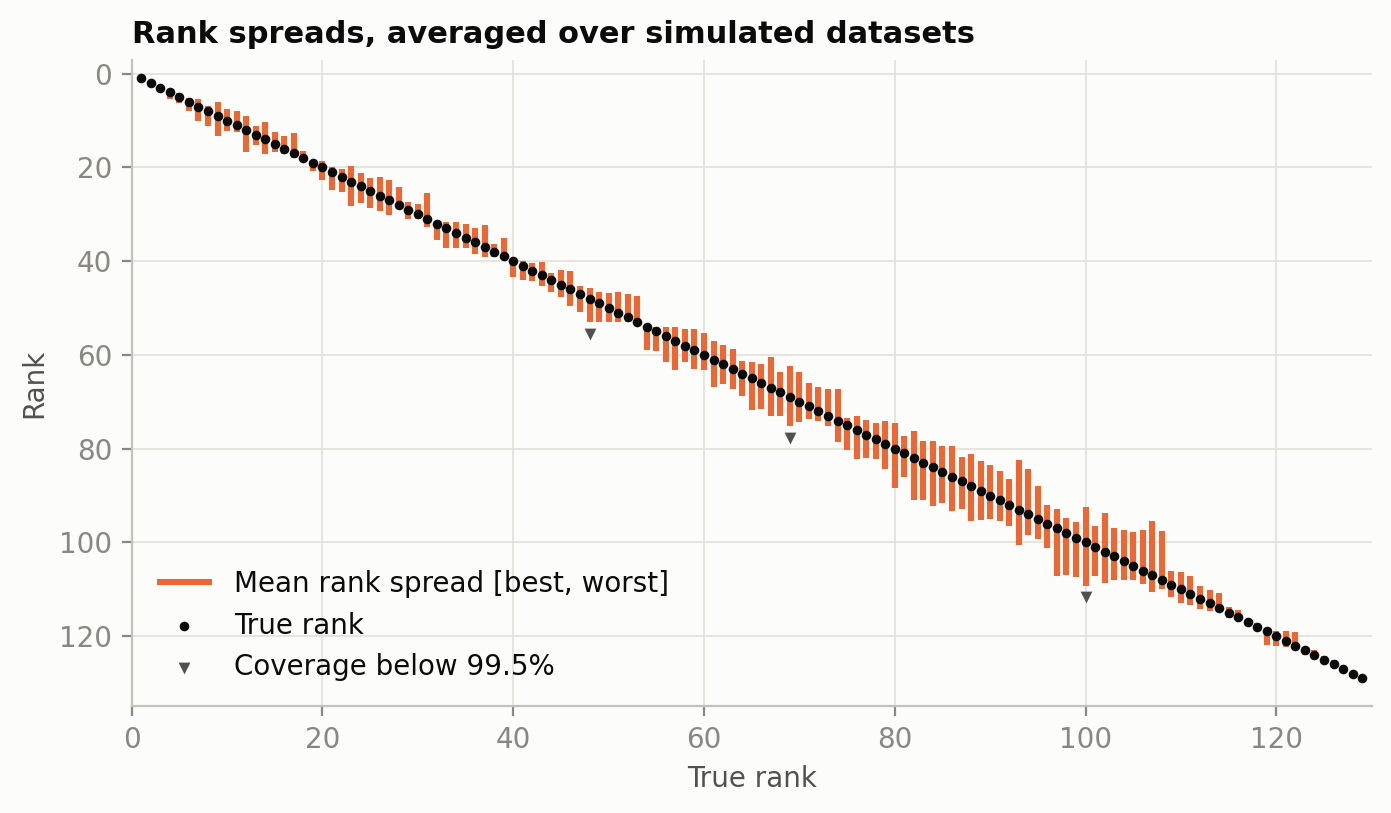
\includegraphics[width=0.82\textwidth]{../docs/figures/q1_spreads.png}
\caption{Mean rank spread of each model over the 1,000 simulated datasets, against its true rank.}\label{fig:q1spreads}
\end{figure}

\subsection{Q2: supplementary results}\label{app:q2}

\begin{table}[h]
\centering\small
\caption{Q2 on the 1,000 datasets of Q1. ``Declared'': orderings the procedure declares; ``rank rule'': pairs whose rank intervals do not overlap. Monte Carlo SEs are below 0.01 for coverage and widths.}\label{tab:q2full}
\begin{tabular}{@{}lrrrrrr@{}}
\toprule
 & \multicolumn{2}{c}{Coverage} & Width & \multicolumn{2}{c}{P(any false ordering)} & True orderings \\
\cmidrule(lr){2-3}\cmidrule(lr){5-6}
Procedure & each & all & (ranks) & declared & rank rule & declared \\
\midrule
Arena & 0.999 & 0.909 & 7.99 & 0.155 & 0.006 & 0.945 \\
Bonferroni & 1.000 & 1.000 & 13.65 & 0 & 0 & 0.901 \\
$\chi^2$ projection & 1.000 & 1.000 & 43.43 & 0 & 0 & 0.669 \\
$\chi^2$ Scheff\'e & 1.000 & 1.000 & 33.07 & 0 & 0 & 0.749 \\
Pairwise Bonferroni & 1.000 & 1.000 & 12.73 & 0 & 0 & 0.908 \\
Holm (one-sided) & 1.000 & 1.000 & 12.38 & 0 & 0 & 0.911 \\
Holm (two-sided) & 1.000 & 1.000 & 11.25 & 0 & 0 & 0.920 \\
\bottomrule
\end{tabular}
\end{table}

Bonferroni's score intervals all cover in $94.5\% \pm 0.7\%$ of datasets, so the union bound is nearly tight for scores; it is the step from scores to ranks that makes Bonferroni conservative.

\begin{table}[h]
\centering\small
\caption{Simultaneous coverage of the rank intervals in the stress-test worlds (1,000 datasets each). Monte Carlo SEs are at most 0.016 (Arena) and 0.006 (others).}\label{tab:stress}
\begin{tabular}{@{}lrrrrr@{}}
\toprule
World & Arena & Bonferroni & Pairwise Bonf. & Holm (1-sided) & Holm \\
\midrule
2024 strengths & 0.909 & 1.000 & 1.000 & 1.000 & 1.000 \\
strengths $\times$ 0.5 & 0.901 & 1.000 & 1.000 & 1.000 & 1.000 \\
strengths $\times$ 0.25 & 0.914 & 1.000 & 1.000 & 1.000 & 1.000 \\
strengths $\times$ 0.1 & 0.915 & 1.000 & 1.000 & 1.000 & 1.000 \\
20 tiers, exactly tied & 0.241 & 1.000 & 0.998 & 0.996 & 0.975 \\
10 tiers, exactly tied & 0.073 & 0.999 & 0.998 & 0.995 & 0.966 \\
20 tiers, spread 5\% & 0.668 & 1.000 & 0.999 & 0.999 & 0.994 \\
20 tiers, spread 10\% & 0.703 & 1.000 & 1.000 & 1.000 & 0.998 \\
20 tiers, spread 20\% & 0.782 & 1.000 & 1.000 & 1.000 & 1.000 \\
all models tied & 0.002 & 0.984 & 0.973 & 0.973 & 0.973 \\
\bottomrule
\end{tabular}
\end{table}

Uniformly scaled-down strengths are not a hard case: the gaps shrink, but so does the number of declared orderings, and few pairs end up close enough to be at risk. A true gap of one standard error makes a wrong-direction rejection at a bar near 4 about 100 times less likely than for a tied pair.

\paragraph{Real board, pair by pair.} Of the 8,256 pairs, Arena's interval rule orders 7,808 and Holm 7,585, all of which Arena also orders. Under the site's rule (rank spreads that overlap count as tied), Arena separates 7,426 pairs; for 428 of them the Holm rank intervals overlap, and none of the 830 pairs Arena shows as tied has separate Holm intervals. Holm agrees with every ordering of Bonferroni's intervals and adds 155. A single-step max-$|z|$ test, with the bar set to the 95th percentile of $\max_{i<j} |Z_i - Z_j| / \SE(\cdot)$ for $Z \sim N(0, \hat V)$ (20,000 draws), separates 7,534 pairs; its step-down version \citep{romano2005exact} stops at a bar of 3.86 and separates 7,603.

\subsection{Q3: supplementary results}\label{app:q3}

\begin{table}[h]
\centering\small
\caption{Q3 categories. Agreement with the official 2024 category boards (128 models) and the pairs tested here.}\label{tab:cats}
\begin{tabular}{@{}llrrrr@{}}
\toprule
Category & Battle belongs when & Battles & Within $\pm$10 & Tested & Bonferroni \\
\midrule
Coding & code detected & 316,372 & 98 & 128 & 35 \\
Math & math tag & 214,348 & 98 & 126 & 40 \\
Instruction following & IF tag (score $\ge 4$) & 581,492 & 97 & 129 & 42 \\
Hard prompts & $\ge 6$ of 7 criteria tags & 447,819 & 98 & 129 & 39 \\
Chinese & language & 176,016 & 100 & 115 & 46 \\
Russian & language & 143,973 & 99 & 95 & 32 \\
Multi-turn & more than one turn & 244,413 & 98 & 128 & 22 \\
Long query & $\ge 500$ user tokens & 164,230 & 99 & 108 & 19 \\
\bottomrule
\end{tabular}
\end{table}

For the tested pairs, our category-minus-overall ratings have correlation at least 0.999 with the official ones. Below 200 battles a few old models disagree with the official category boards by up to 408 points; the official values look like a non-converged fit (three Russian models share an identical rating), which is one reason for the 200-battle minimum. The sizes of the global tests under the null, estimated from fresh draws, are 0.06 (HC), 0.05 (HC$^+$), 0.05 (min-$P$) and 0.08 ($\chi^2$). In the power simulation BH's false discovery proportion ranges from 0.01 to 0.12 across the grid, often well below 10\%, and Bonferroni's probability of any false discovery is 6.5\% with no specialties and at most 9\% on the grid, a little above 5\%, probably because each null SD is estimated from 500 draws. Categories overlap (many coding battles are also hard prompts), so a specialty planted in one category also moves the model in overlapping categories; such discoveries (1--23\%) are counted separately as spillovers, not as false.

\begin{figure}[h]
\centering
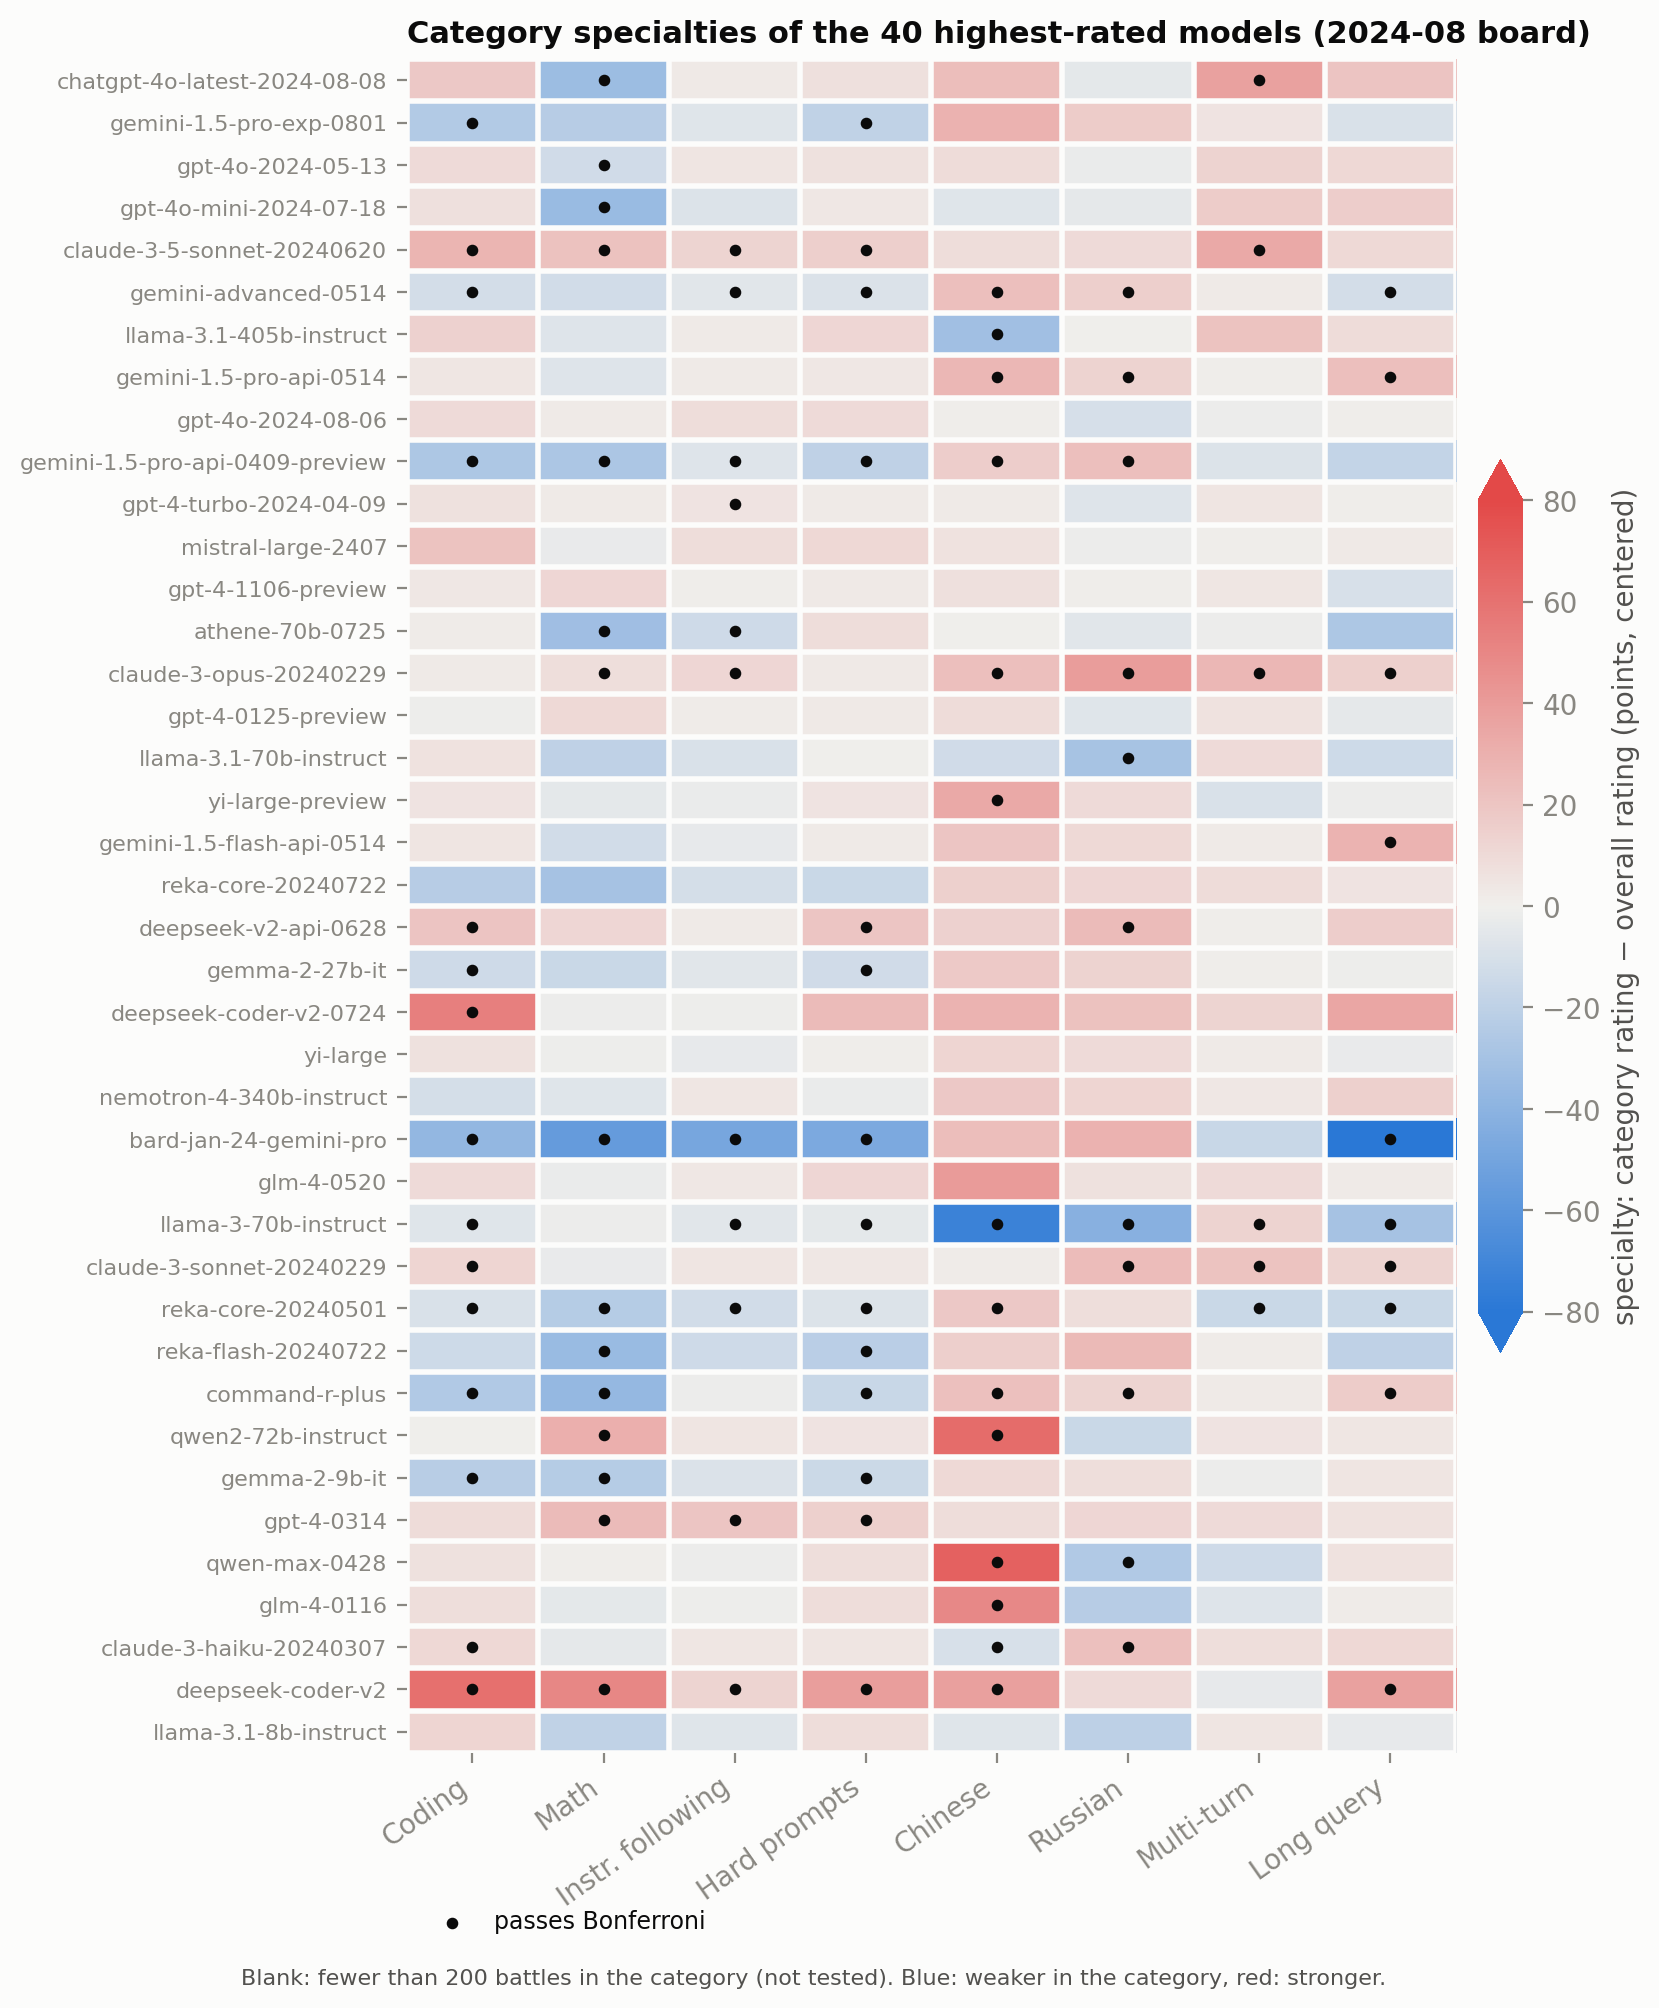
\includegraphics[width=0.66\textwidth]{../docs/figures/q3_specialties.png}
\caption{Estimated specialties (category rating minus overall rating, centered within the category) of the 40 highest-rated models; dots mark pairs that pass Bonferroni.}\label{fig:q3map}
\end{figure}

\end{document}
